\documentclass[11pt,twocolumn,letterpaper]{article}

%\usepackage{cvpr}
\usepackage{subfig}
\usepackage{times}
\usepackage{epsfig}
\usepackage{graphicx}
\usepackage{amsmath}
\usepackage{lipsum}
\usepackage{amssymb}
\usepackage[british]{babel}
\usepackage[backend=biber, style=ieee]{biblatex}
\usepackage{url}
\usepackage[bookmarks=true]{hyperref}
\usepackage[noabbrev,capitalise]{cleveref}
\usepackage{appendix}
\usepackage{booktabs}
\bibliography{biblio}

\captionsetup[figure]{font=small}

\begin{document}
	
	%%%%%%%%% TITLE
	\title{Chord: A Scalable Peer-to-peer Lookup Protocol for Internet Applications}
	
	\author{Alessandro Cacco\\
		mat. 203345\\
		{\tt\small alessandro.cacco@studenti.unitn.it}
		\and
		Andrea Ferigo\\
		mat. 207486\\
		{\tt\small andrea.ferigo@studenti.unitn.it}
		\and
		Enrico Zardini\\
		mat. 207465\\
		{\tt\small enrico.zardini@studenti.unitn.it}
	}
	\date{}
	\maketitle
	
	\section{Introduction}
	\label{sec:intro}
	This work aims at illustrating an implementation of Chord, a scalable distributed lookup protocol described in \cite{chord}. Basically, Chord provides a primitive, i.e. \textit{lookup}, that allows to determine the responsible for a key in an efficient way. Hence, it represents a great solution to the data location problem: each data item needs just to be associated with a key and stored in the node to which the key is mapped. \newline 
	In practice, the nodes are logically arranged in a ring topology and each of them is responsible for the ids belonging to the interval $(predecessorId, nodeId]$ \footnote{The ids are integers in $[0,2^m)$, where $m$ is the number of bits of the identifiers. All the arithmetic is modulo $2^m$.}. The key-data pairs are assigned to the nodes depending on the hash value of the key and consistent hashing is used in order to keep the load balanced. Moreover, each node is required to maintain information about only a few other nodes: the predecessor, some successors and the elements of the finger table\footnote{The finger table is a routing table: the $i^{th}$ entry points at the responsible for the identifier $nodeId+2^{i-1}$, with $1\leq i \leq$ m.\label{foot:ftable}}. Therefore, Chord scales well to large numbers of nodes without affecting performance. Actually, it adapts effectively also in dynamic environments with frequent joins and leaves thanks to a simple stabilization algorithm. \newline
	Finally, it is worth mentioning that the iterative version of Chord has been implemented. Hence, a node resolving a lookup initiates all the communications needed to reach the target. \newline
	Starting from this, \cref{sec:implementation} will describe in detail the implementation, \cref{sec:simulator} will present how to run the simulator and illustrate the view that has been developed to show the protocol's functioning, \cref{sec:analyses} will describe the simulations that have been performed and analyse the results obtained. \newline
	The source code is available at \url{https://github.com/ZarHenry96/DS2-A2}. 
	
	\section{Implementation}
	\label{sec:implementation}
	This section presents the methods and the behaviour of the five classes that have been used to implement the protocol. In particular, these classes can be subdivided into three groups:
	\begin{itemize}
		\item the control class (\texttt{TopologyBuilder}) that instantiates the nodes, initialises the ring, manages joins/leaves and initiates the lookups;
		\item the class (\texttt{Node}) that defines the behaviour of the agents in the simulation, i.e. the nodes;
		\item the support classes (\texttt{FingerTable}, \texttt{Lookup} and \texttt{Utils}).
	\end{itemize}
	Before going into details, it is worth highlighting that the correspondence between simulation ticks and seconds has been assumed in both implementation and simulations. 
	
	\subsection{TopologyBuilder}
	\label{subsec:topbuilder}
	As introduced in the previous section the \texttt{TopologyBuilder} has several duties, which can be grouped into two phases: initialization and scheduling. During the first one it initialises the nodes and generates the data. Instead, in the second one it schedules insertions/leavings and lookups.
	
	\subsubsection{Initialization}
	\label{subsubsec:top-init}
	The first thing the \texttt{TopologyBuilder} does is initialise the ring with a certain number of nodes, which is defined by the parameter \textit{init\_num\_nodes}. Actually, the ring can be initialised in two different ways\footnote{It is possible to change the mode using the parameter \textit{one\_at\_time\_init}.}. As regards the first one, the nodes are inserted one at a time providing them with a reference to a random node already present in the network. In particular, between two consecutive insertions the \texttt{TopologyBuilder} waits a certain number of ticks, which is defined by the parameter \textit{insertion\_delay} \footnote{The \textit{insertion\_delay} is always greater than the maximum time needed for a stabilization, i.e. there is always a stabilization round between two consecutive insertions}. It is also worth mentioning that the first inserted node does not execute the \textit{join()} method, but the \textit{create()} one, as highlighted in \cref{subsubsec:init}. As for the other mode, all \textit{init\_num\_nodes} nodes are inserted at the same time without any delay. Moreover, each of them is provided with the right immediate successor in order to start the simulation with a ring that has already reached a stable state. Hence, no \textit{create()} or \textit{join()} method is called; instead, \textit{initSuccessor()} is used. \newline
	The second thing that the \texttt{TopologyBuilder} does during the initialization is the generation of the key-data pairs, which is performed after a stabilisation round since the last insertion. In particular, the \texttt{TopologyBuilder} creates the data according to 3 parameters: \textit{data\_size}, \textit{key\_size} and \textit{total\_number\_data} which correspond to the size of the random strings that represent the data, the size of the sub-strings used as keys, and the total number of data stored in the ring, respectively\footnote{Note that the sizes indicate the number of characters. Moreover, it is important to highlight that there cannot be more than $2^m$ data.}. At the end of the data generation, the \texttt{TopologyBuilder} assigns each key to the first active node that has an id greater than or equal to the hash value of the key\footnote{Clearly, all the keys greater than the id of the last active node are assigned to the node with the smallest id in order to respect the modular structure of the ring.}.
	
	\subsubsection{Scheduling}
	\label{subsubsec:top-scheduling}
	At the end of the initialization, the \texttt{TopologyBuilder} schedules two types of functions:
	\begin{itemize}
		\item the functions managing the leaving/insertion process (\textit{leaving\_nodes()} and \textit{join\_new\_nodes()});
		\item the function initiating the lookups (\textit{lookupSingleKey()} or \textit{lookupMultipleKeys()})
	\end{itemize}
	As regards the first type, the leavings are scheduled every \textit{leave\_interval} ticks starting after one stabilization since the last insertion. In particular, a set of active nodes\footnote{The number of nodes leaving the ring is given by the combination of two parameters: \textit{min\_number\_leaving} and \textit{leaving\_amplitude}.} is randomly selected every time and their leavings are scheduled at a distance of one tick from each other. This is done in order to allow the nodes to notify the neighbours and to transfer the data. Then, after \textit{join\_interval} ticks since the last leaving, the insertion procedure is started. Analogously, a set of random inactive nodes\footnote{The number of nodes joining the ring is given by the combination of \textit{min\_number\_joins} and \textit{join\_amplitude}.} is selected; however, in this case, unlike the leavings and the initialization phase, the insertions are concurrent, i.e. there is no delay between them. \newline
	Actually, it is worth mentioning that this is not the only way a node can leave the ring: as described in \cref{subsubsec:leaving}, a node may be forced to leave due to the lack of alive successors. In that case, it is removed from the active nodes by the \texttt{TopologyBuilder} and an additional join is scheduled at the next insertion round.\newline
	As regards the lookups, the procedure is very similar: every \textit{lookup\_interval} ticks since the data generation, the \texttt{TopologyBuilder} schedules the initiation of \textit{number\_lookup} queries\footnote{In case the number of alive nodes is less than \textit{number\_lookup}, all of them initiate only one query, since a node can perform only one lookup at a time (for graphical reasons).}. Actually, there are two different lookup modes: all nodes look for the same key (\textit{lookupSingleKey()}); every node looks for a random key (\textit{lookupMultipleKeys()}) \footnote{The mode is defined by the parameter \textit{one\_key\_lookup}.}.
	
	
	\subsection{Node}
	\label{subsec:node}
	The \texttt{Node} class, which defines the behaviour of the agents in the simulations, consists of several methods that can be grouped into six categories:
	\vspace{-2pt}
	\begin{itemize}
		\itemsep0pt
		\item initialization;
		\item lookup;
		\item stabilization;
		\item data management;
		\item crash and recovery;
		\item leaving.
	\end{itemize}
	\vspace{-1pt}
	Each of them will be examined in a specific Section. As regards the main fields, every node maintains: a finger table (the implementation will be presented in \cref{subsubsec:finger-table}), a list of successors, a reference to the predecessor and a key-value map for data. \newline
	Basically, the finger table - as a routing table - allows to perform efficient and scalable lookups. In fact, the finger table is not needed for correctness\footnote{It is sufficient that every node knows its successor to achieve correctness.} but avoids lookups characterised by a number of messages linear in the number of nodes. \newline
	Instead, the list of successors improves the robustness to failures and departures w.r.t. just a reference to the immediate successor. In fact, all successors would have to fail simultaneously in order to destroy the ring. It is worth mentioning that the first element of the finger table and the first element of the successor list coincide. \newline
	As regards the reference to the predecessor, it is exploited by the stabilization algorithm to maintain the consistency of the successors and is used to transfer part of the data to the new responsible in presence of a join.
	
	\subsubsection{Initialization}
	\label{subsubsec:init}
	As described in \cref{subsec:topbuilder}, two ring initialization modes are supported: the insertion of one node at a time until the desired size has been reached; the creation of a ring of the desired size in which each node knows the immediate successor. \newline
	The former is supported by the \textit{create()} and \textit{join()} methods: \textit{create()} is called on the first node in order to build a new Chord ring, whereas \textit{join()} performs all the operations required to join an existing ring. Hence, \textit{join()} is used also after the initial phase of the simulation to insert new nodes in the ring. \newline
	Instead, the latter is supported by the \textit{initSuccessor()} method, which initialises the successor list using the node provided. \newline
	As regards joining an existing ring, it implies asking a node already contained in the ring for the successor of the current node. This is done through the \textit{find\_successor\_step()} method, which is presented in the following Section.
	
	\subsubsection{Lookup}
	\label{subsubsec:lookup}
	As introduced in \cref{sec:intro}, the lookups are performed in an iterative way. Hence, the node on which the \textit{lookup()} method is called initiates all the communications needed to reach the responsible for the given key. \newline
	Basically, the node first checks if its successor is the responsible for the key of interest: if it is, the lookup is finished; otherwise it asks the closest preceding node (w.r.t. the given key) among the ones contained in the finger table and in the successor list. Since the iterative version has been implemented, if the contacted node's successor is not the responsible, the contacted node provides the lookup initiator with a reference to the closest preceding node among the ones it knows. The procedure is repeated until the responsible is found. \newline
	Since the same steps are performed during the stabilization, the \textit{lookup()} method just calls another function, i.e. \textit{find\_successor()}. In practice, \textit{find\_successor()} does the first check, whereas the \textit{find\_successor\_step()} method implements the iterative step. As regards the communications between nodes, they are performed through the methods \textit{processSuccRequest()} and \textit{processSuccResponse()} using an exponentially distributed packet delay with mean of 50 milliseconds (0.05 ticks) as in \cite{chord}. \newline
	Actually, the lookup initiator may not receive an answer due to a failure or an out-of-date reference (the target node has left the ring). In that case, after 500 milliseconds (0.5 ticks) it contacts the node from which it has learnt about that node in order to obtain another reference (\textit{getPrevSuccessor()} method). If that node does not reply either, the lookup initiator iterates the procedure.
	
	\subsubsection{Stabilization}
	\label{subsubsec:stabilization}
	The stabilization protocol is run periodically to ensure that the various pointers (finger table, successors, predecessor) are up-to-date. The main method is \textit{stabilization()}, which starts the various operations. \newline
	First of all, the node contacts sequentially its successors until it finds one alive (this is done in \textit{stabilization()}). At that point, if the predecessor of the replying node belongs to the interval $(nodeId,successorId)$ the current node updates its immediate successor (\textit{stabilization\_step()} method) \footnote{This may happen in case a new node has recently joined the ring.}. The next step consists in asking the immediate successor for its successor list, which is used to update the list of the current node. As regards this communication, it is managed through the methods \textit{processStabRequest()} and \textit{processStabResponse()}. In particular, the first method also verifies if the predecessor of the contacted node needs to be changed  (\textit{notifiedPredecessor()} method). In that case, the contacted node transfers the necessary data -if any- to the new predecessor (current node) and notifies the old predecessor that its successor should be changed (\textit{setNewSuccessor()} method) accelerating the integration of the new node in the ring. \newline
	Once the response has been processed, the node moves on to the stabilization of the other pointers. This is done by the \textit{fix\_data\_structures()} method: basically, the node stabilizes alternatively one entry of the finger table (\textit{fix\_fingers()} method) and one entry of the successor list (\textit{fix\_successors()} method) in addition to the predecessor. As regards the finger table, the node calls the \textit{find\_successor()} method in order to find the responsible for the id the entry points to. Instead, as for the successor list, the node calls the same method on the id of the last stabilized successor plus one ($mod\ 2^m$). Once the responsible has been found, the corresponding data structure is updated by the \textit{setResult()} method. In particular, since the first entry of the two data structures represents the immediate successor, they are never stabilized during this phase (it has already been done in the previous one). Finally, the node checks if the predecessor is still alive: if it is not, the pointer is set to \texttt{null}, which allows the node to accept a new predecessor in the next stabilization.
	
	\subsubsection{Data management}
	\label{subsubsec:data-management}
	The data management category includes two methods: \textit{transferDataUpToKey()} and \textit{newData()}. \newline
	Basically, the former extracts the data with a hash value of the key up to a target value from the data owned by the current node, whereas the latter performs the acquisition of new data. In practice, these methods are exploited to transfer data: to the new predecessor; to the successor before leaving the ring (this operation is managed by the \texttt{TopologyBuilder}). 
	
	\subsubsection{Crash and recovery}
	\label{subsubsec:crash-n-recovery}
	Nodes failures are simulated as follows: each node periodically crashes with a certain probability (\textit{nodeCrash()} method) and schedules the recovery after a specific interval (\textit{recovery()} method). While failed the node does not process any request or response. Instead, once it is up again, it performs immediately a stabilization using the references it had before crashing.
	
	\subsubsection{Leaving}
	\label{subsubsec:leaving}
	As described in \cref{subsubsec:top-scheduling}, nodes leavings are decided and scheduled by the \texttt{TopologyBuilder}. However, all the operations that a node has to perform before leaving the ring are implemented in the \textit{leave()} method
	of the \texttt{Node} class. \newline
	Basically, the node contacts first the immediate successor notifying it of the departure and providing it with the new predecessor -if it is not \texttt{null}- and the data the current node is holding (\textit{setPredecessor()} and \textit{newData()} methods). Then, it contacts the predecessor providing it with its immediate and last successor, which are used to update the successor list of the predecessor node (\textit{setLastSuccessor()} method). At that point, the node can safely leave the ring and clear all its data structures (\textit{clearAll()} mehtod). \newline
	Actually, a node may also be forced to leave the ring. In fact, if during a stabilization or a lookup operation it realizes that all its successors are failed or have left the ring, it is forced to leave the ring. This is managed by the \textit{forcedLeaving()} method, which notifies the predecessor of the departure (\textit{successorLeaving()} method), clears all the data structures and communicates the leaving to the \texttt{TopologyBuilder} that will insert an additional node in the next join round.
	
	\subsection{Support classes}
	\label{subsec:support-classes}
	This section briefly describes the structure of the three classes that support the operations of \texttt{TopologyBuilder} and \texttt{Node}, i.e.: \texttt{FingerTable}, \texttt{Lookup} and \texttt{Utils}.
	
	\subsubsection{FingerTable}
	\label{subsubsec:finger-table}
	The \texttt{FingerTable} class defines the structure of the finger table, which is nothing more than a routing table, as described in \cref{foot:ftable}. In practice, the finger table has been implemented as an hash-map: the key corresponds to the index of the routing table, whereas the value is the reference to the pointed node. Moreover, the \texttt{FingerTable} class provides all the necessary methods to interact with the finger table, such as \textit{getEntry()}, \textit{setEntry()}, \textit{getKeys()}, \textit{removeEntry()} etc.
	
	\subsubsection{Lookup}
	\label{subsubsec:lookup-class}
	The \texttt{Lookup} class provides a useful structure for keeping track of the information related to a specific lookup. \newline
	In particular, when the \texttt{TopologyBuilder} initiates a lookup, it creates a new instance of the \texttt{Lookup} class providing information such as the hash value of the target key, the id of the node performing the lookup, the starting tick and the correct result (id of the responsible node). \newline
	Once the lookup has been finished, the lookup initiator calls the \textit{setResult()} method on the corresponding \texttt{Lookup} instance providing the result information, i.e. the reference to the node responsible for the target key, the path length, the number of timeouts experienced and the number of nodes contacted. At that point, a check to verify if the right node has been found and it has effectively the key is performed.
	
	\subsubsection{Utils}
	\label{subsubsec:utils}
	The \texttt{Utils} class provides three static utility methods: \textit{getHash()}, \textit{getNextDelay()} and \textit{belongsToInterval()}. \newline
	The first one computes the hash value of the key provided (SHA-1 is used). The second one returns a random delay taken from an exponential distribution with mean equal to the one supplied. The last one verifies if the value provided belongs to the interval defined by the endpoints supplied in modular arithmetic.
	
	\section{Simulator}
	\label{sec:simulator}
	This section deals with how to run the simulations and presents the view that has been developed to show the protocol's functioning.
	
	\subsection{Guide to the simulator}
	\label{subsec:simulator-guide}
	In order to execute the simulator, the first step consists in importing the project. After that, the \textit{Chord} model has to be run: the default graphic interface of Repast Symphony will be shown. At that point, the simulation parameters can be set in the \textit{Parameters} panel. In particular, the initialisation strategy is determined by the checkbox labelled as \textit{Init - initialise the ring one node at a time}.  Instead, the \textit{Scenario Tree} panel allows to select the data to be saved \texttt{(Data Sets} item) and the location (\texttt{Text Sinks} item). As regards the former, it is possible to choose the methods to call on the agents and the time to do that. As for the latter, the data set fields to be stored in the file can be selected. Actually, the lookup results are saved in a different way: in fact, at the end of the simulation the \texttt{TopologyBuilder} writes the collected data to a file through the method \textit{getLookupsResults()} (this behaviour is defined at the end of the \textit{build()} method of the same class). Once all this has been done, it is possible to start the simulation, which can be paused or stopped at a specific tick by setting the corresponding value in the \texttt{Run Options} panel.
	
	\subsection{Simulation view}
	\label{subsec:simulation-view}
	The view that is shown during the execution of the simulation displays in real-time the nodes in the Chord ring and their status. In particular, the view shows for each node: the id, the content of the finger table, the immediate successor, the predecessor and the lookup key (if any, during a lookup). For what concerns the node's colour, orange means not yet initialized, i.e. the successor has not yet become aware of it\footnote{This implies that the node is not yet part of the ring, since nobody is aware of it.}, green corresponds to initialized and functioning, red signifies crashed. Actually, the view shows also the communications between nodes during a lookup batch through violet arrows: basically, each arrow goes from the lookup initiator to the contacted node; in case the contacted node has already left the ring, the arrow points to an empty space.
	
	\section{Analyses and Results}
	\label{sec:analyses}
	This section presents the simulation runs that have been executed to test the protocol strength and performance, with their respective analyses and results explanations. The parameters involved in our simulations are explained in \cref{tab:default_params}, with the corresponding default parameters. The performed runs are designed with variations on the default parameters so four analyses are possible, namely:
	\begin{itemize}
		\item Crash probability analysis (\cref{subsec:crash_analysis}), in order to understand the impact of having a higher number of nodes crashing during the protocol, causing errors in the other nodes data structures;
		\item Network size analysis (\cref{subsec:netsize_analysis}), with proportioned lookup batch sizes, allows both for scaling testing and for lookup load stress-testing;
		\item Key number analysis (\cref{subsec:keyno_analysis}), testing the scaling performance of the protocol wrt the number of keys in the system
	\end{itemize}
	
	\begin{table}[!ht]
		\caption{Default protocol parameters for the executed experimental runs.}
		\label{tab:default_params}
		\centering
		\begin{tabular}{lc}
			\hline
			\textbf{Parameter} & \textbf{Value} \\
			\hline
			Crash probability & 0.05\\
			\hline
			Crash recovery interval & 25\\
			\hline
			Crash scheduling interval & 60\\
			\hline
			Key size & 5 \\
			\hline
			Number of keys & 1500\\
			\hline
			Value size & 10\\
			\hline
			Hash size & 12\\
			\hline
			Initial number of nodes & 1000\\
			\hline
			Successors list & 20\\
			\hline
			Join tick period & 20\\
			\hline
			Join amplitude & 0\\
			\hline
			Join min number of nodes & 10\\
			\hline
			Leave tick period & 50\\
			\hline
			Leave amplitude & 0\\
			\hline
			Leave min number of nodes & 10\\
			\hline
			Lookup period & 35\\
			\hline
			Lookups per batch & 500\\
			\hline
			Single key lookup & no\\
			\hline
			Stabilization amplitude & 1\\
			\hline
			Stabilization period & 15\\
			\hline
		\end{tabular}
	\end{table}
	
	\subsection{Impact of crashing nodes}
	\label{subsec:crash_analysis}
		\Cref{tab:crash_runs} lists the runs performed in order to analyse the impact of higher percentages of crashing nodes. First of all, the plot in \Cref{fig:crash0} validate the experimental runs, as we can see how the number of nodes is consistent throughout each run, with a reasonable expected difference between them. 
						
		\begin{table}[h!]
			\caption{Variations of the default parameters for the node crashing impact analysis. Note that \texttt{R01} is the default run with no variations}
			\label{tab:crash_runs}
			\centering
			\begin{tabular}{cc}
				\hline
				\textbf{Run} & \textbf{Crash probability}\\
				\hline
				\texttt{R01} & $0.05$\\
				\hline
				\texttt{R02} & $0.1$\\
				\hline
				\texttt{R03} & $0.2$\\
				\hline
				\texttt{R04} & $0.3$\\
				\hline
			\end{tabular}
		\end{table}
		\begin{figure}[h]
			\centering
			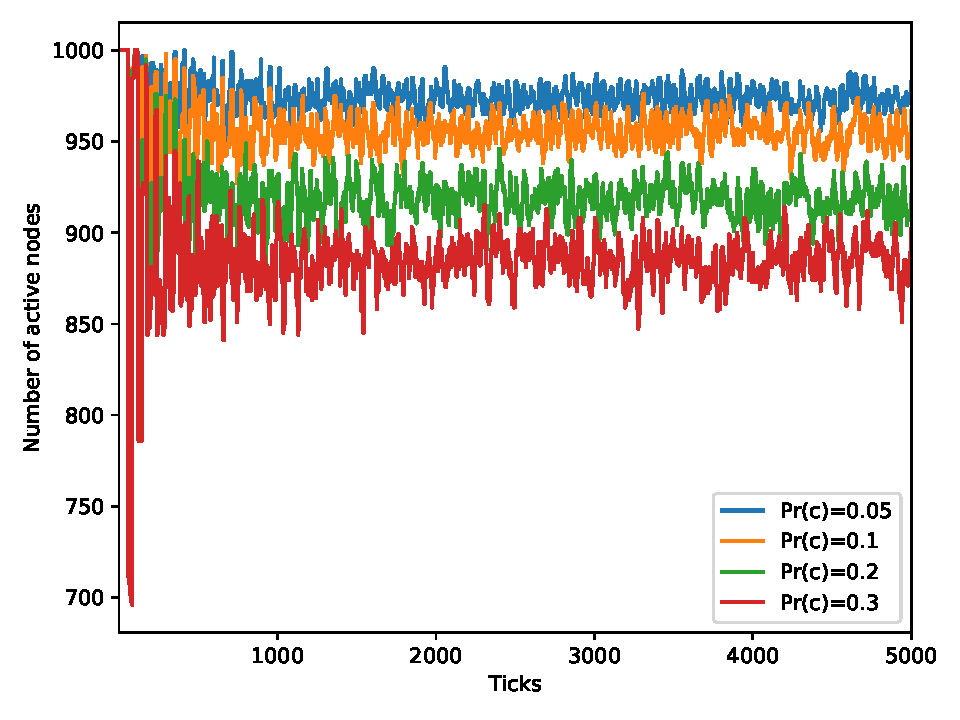
\includegraphics[width=\linewidth,clip,trim=0 0.5cm 0 0.35cm]{figures/analysis1/nodesup_time.pdf}
			\caption{Number of working nodes throughout the runs}
			\label{fig:crash0}
		\end{figure}

		The plots (\Cref{fig:crash1,fig:crash2,fig:crash3,fig:crash4,fig:crash5,fig:crash6}) clearly shows how the protocol is resistant even to a third of the total nodes periodically experiencing a sudden crash. Particularly, \Cref{fig:crash1} shows how the number of steps needed for a lookup slightly increases in mean and variance with the crashing probability, consequently increasing the average lookup duration which quickly stabilizes after an initial transient state, as can be observed in \Cref{fig:crash2}. 

		\begin{figure}[!h]
			\centering
			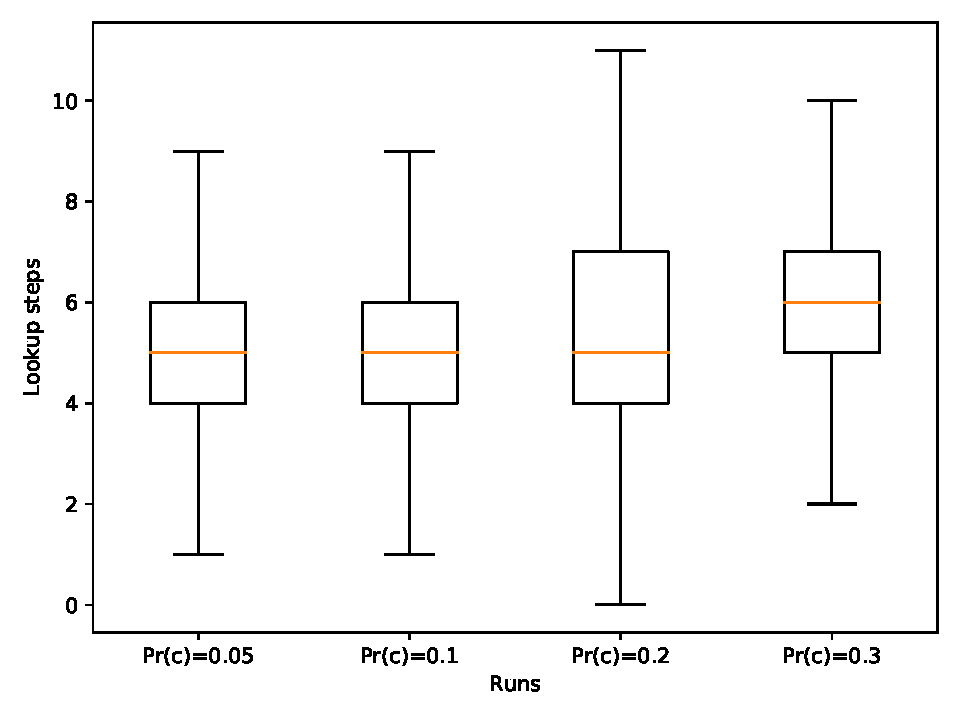
\includegraphics[width=\linewidth,clip,trim=0 0.5cm 0 0.35cm]{figures/analysis1/lookuplength_box.pdf}
			\caption{Boxplot showing the number of steps needed to complete a lookup for each run}
			\label{fig:crash1}
		\end{figure}
		\begin{figure}[!h]
			\centering
			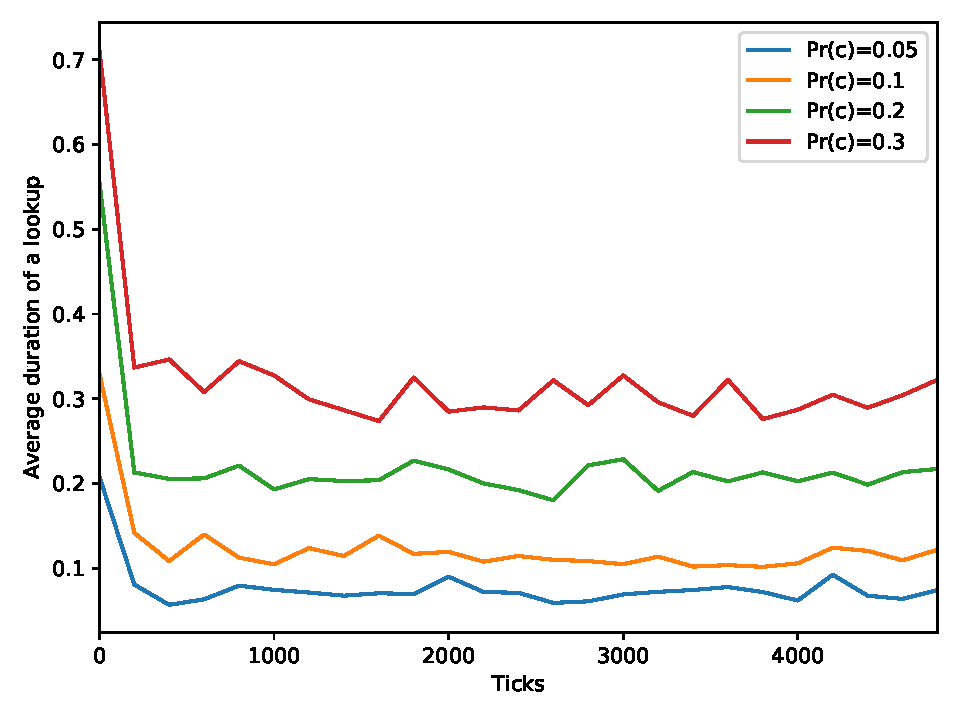
\includegraphics[width=\linewidth,clip,trim=0 0.5cm 0 0.35cm]{figures/analysis1/lookupduration_time.pdf}
			\caption{Average duration of lookups throughout each run}
			\label{fig:crash2}
		\end{figure}

		Furthermore, \Cref{fig:crash3} confirms that lookups takes longer due to a higher quantity of contacted nodes, not because the lookups find valid fingers, value which also stabilizes after an initial transient state (around $\sim400$ ticks) as shown in \Cref{fig:crash4}. The crash probability parameter has also an impact on the number of timeout which are experienced by a lookup, in particular in the initial phase of the protocol in which the data structures are not yet fully populated (see \Cref{fig:crash5}). 

		\begin{figure}[!h]
			\centering
			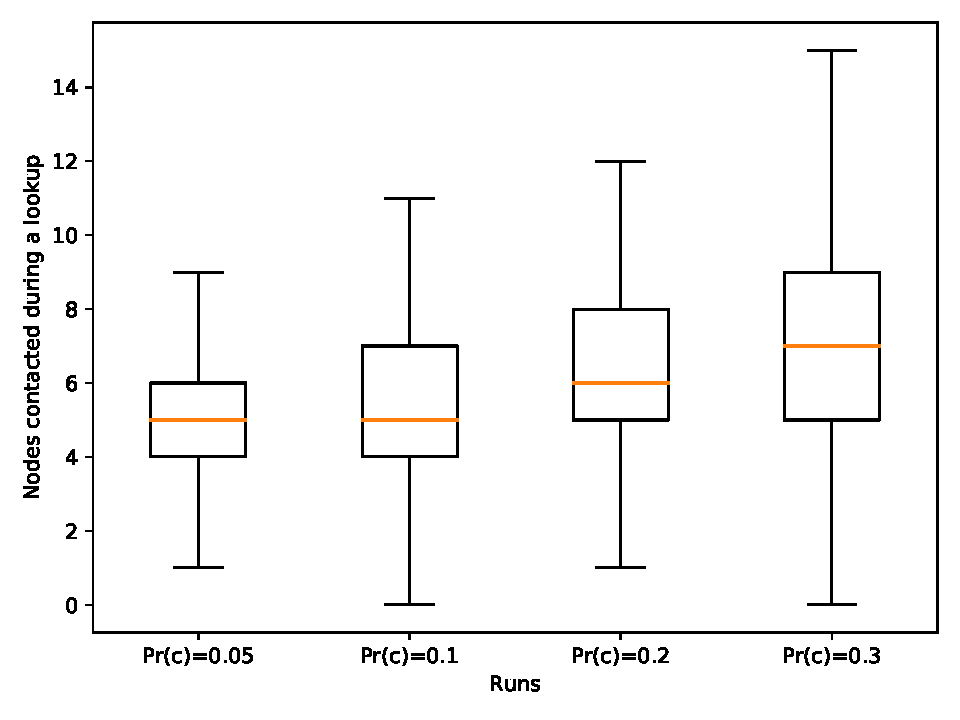
\includegraphics[width=\linewidth,clip,trim=0 0.5cm 0 0.35cm]{figures/analysis1/nodescontacted_box.pdf}
			\caption{Boxplot of the number of nodes contacted to complete a lookup for each run}
			\label{fig:crash3}
		\end{figure}
		\begin{figure}[!h]
			\centering
			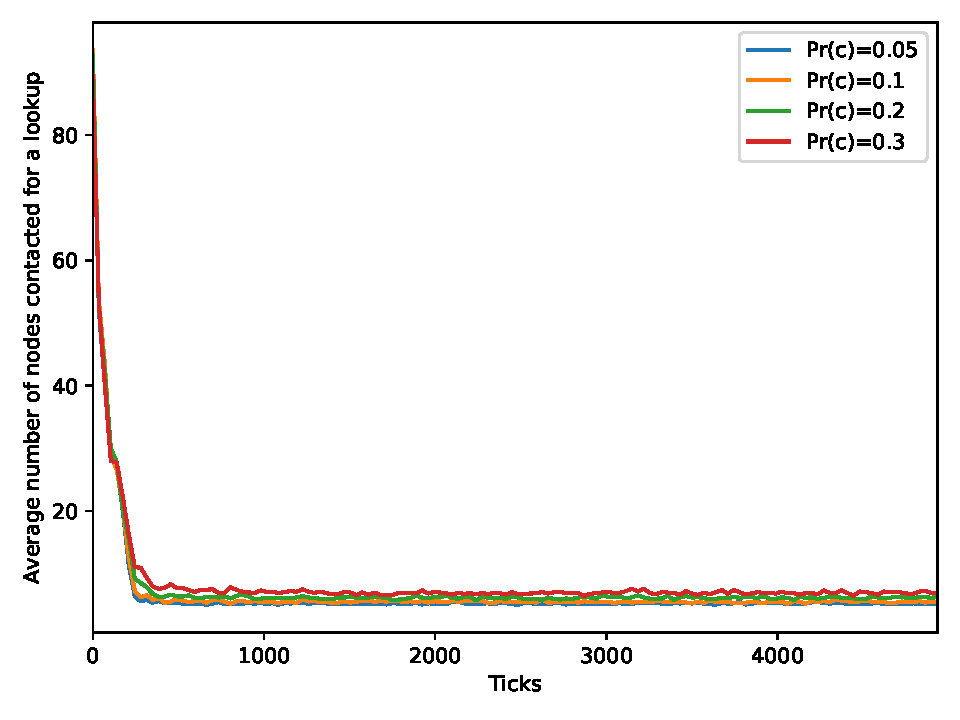
\includegraphics[width=\linewidth,clip,trim=0 0.5cm 0 0.35cm]{figures/analysis1/nodescontacted_time.pdf}
			\caption{Average number of nodes contacted for a lookup throughout each run}
			\label{fig:crash4}
		\end{figure}
		\begin{figure}[!h]
			\centering
			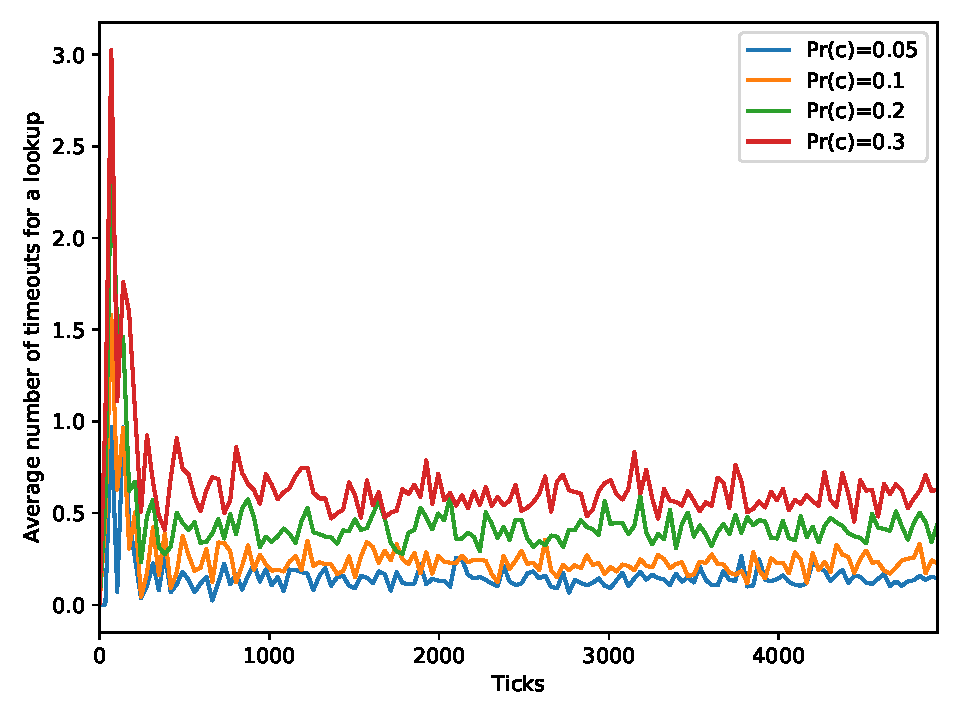
\includegraphics[width=\linewidth,clip,trim=0 0.5cm 0 0.35cm]{figures/analysis1/timeouts_time.pdf}
			\caption{Timeouts experienced by nodes during lookups throughout each run}
			\label{fig:crash5}
		\end{figure}

		Intuitively, a higher crashing probability should cause more lookup failures, however the protocol resistance is again shown in \Cref{fig:crash6}, where the number of failed lookups ($\sim4\times10^1$) is negligible wrt the total number of lookups ($\sim7\times10^4$). 

		\begin{figure}[!h]
			\centering
			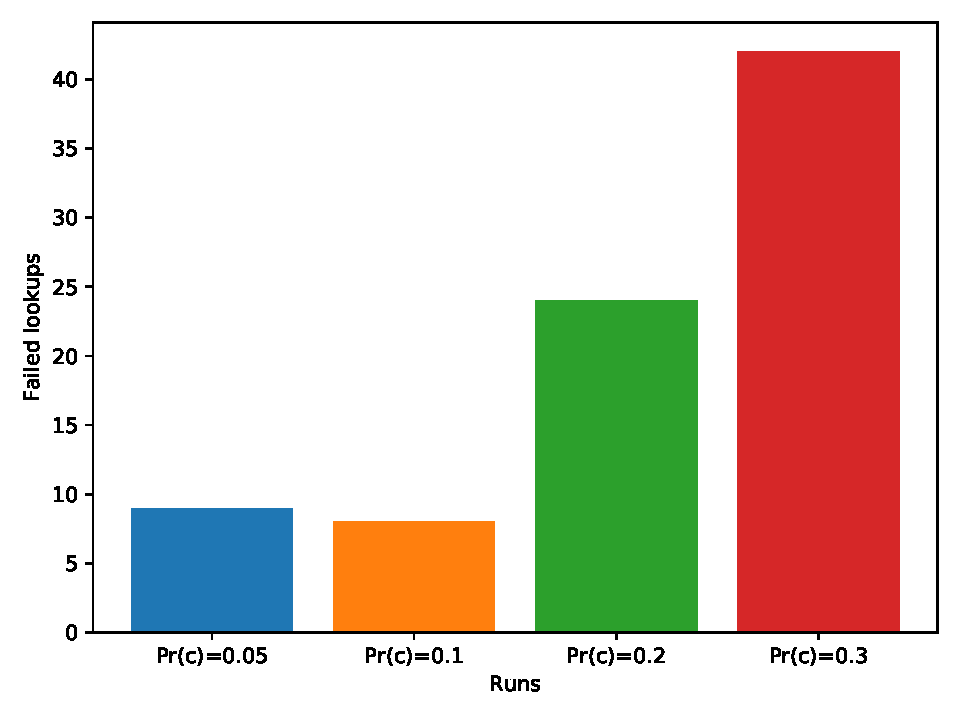
\includegraphics[width=\linewidth,clip,trim=0 0.5cm 0 0.35cm]{figures/analysis1/failedlookups.pdf}
			\caption{Number of failed lookup. Note that the total number of lookups for these runs is $\sim7\times10^4$}
			\label{fig:crash6}
		\end{figure}
	
		An interesting analysis is the one presented in \Cref{fig:crash7}, where the number of error present in the nodes data structures can be observed. As expected, a greater quantity of crashing nodes implies more errors, which are still contained and constant throughout the runs.
		
		\begin{figure}[!h]
			\centering
			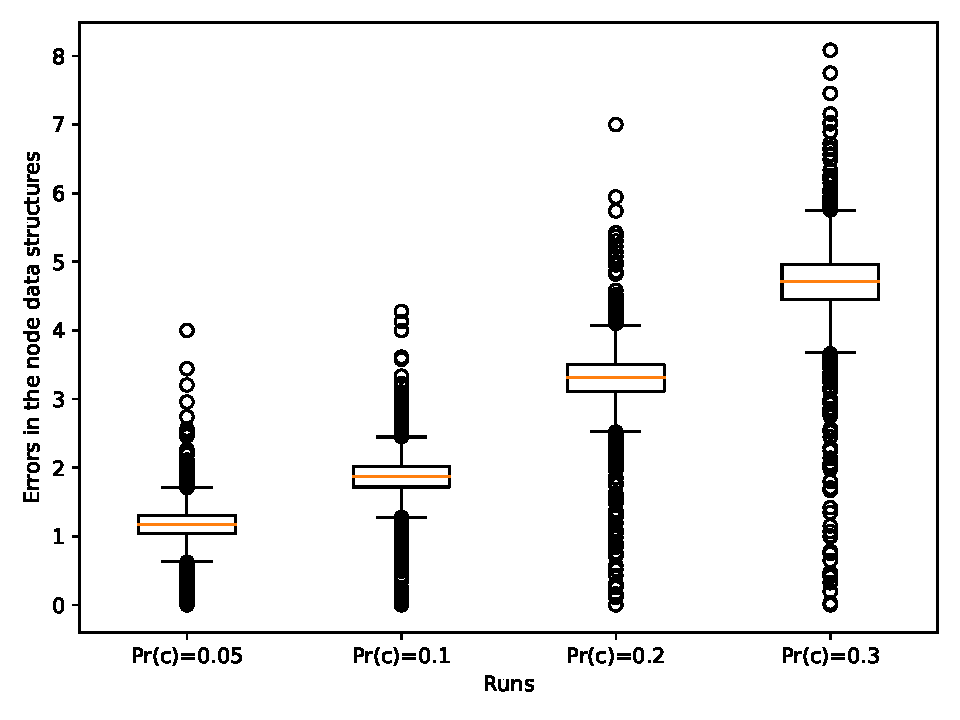
\includegraphics[width=\linewidth,clip,trim=0 0.5cm 0 0.35cm]{figures/analysis1/errors_box.pdf}
			\caption{Average number of errors in the a node data structures, i.e. caused by nodes that unsubscribed or crashed while being in the finger table and/or in the successors list of another node. Considering runs with different crash probabilities.}
			\label{fig:crash7}
		\end{figure}
	
	\subsection{Protocol network size scaling}
	\label{subsec:netsize_analysis}
	Further tests have been performed in order to verify the scalability of the algorithm, with the runs listed in \Cref{tab:netsize_runs}. Several parameters have been varied parallelly, so that the values matches meaningful realistic situations. 


	\begin{figure}[!ht]
		\centering
		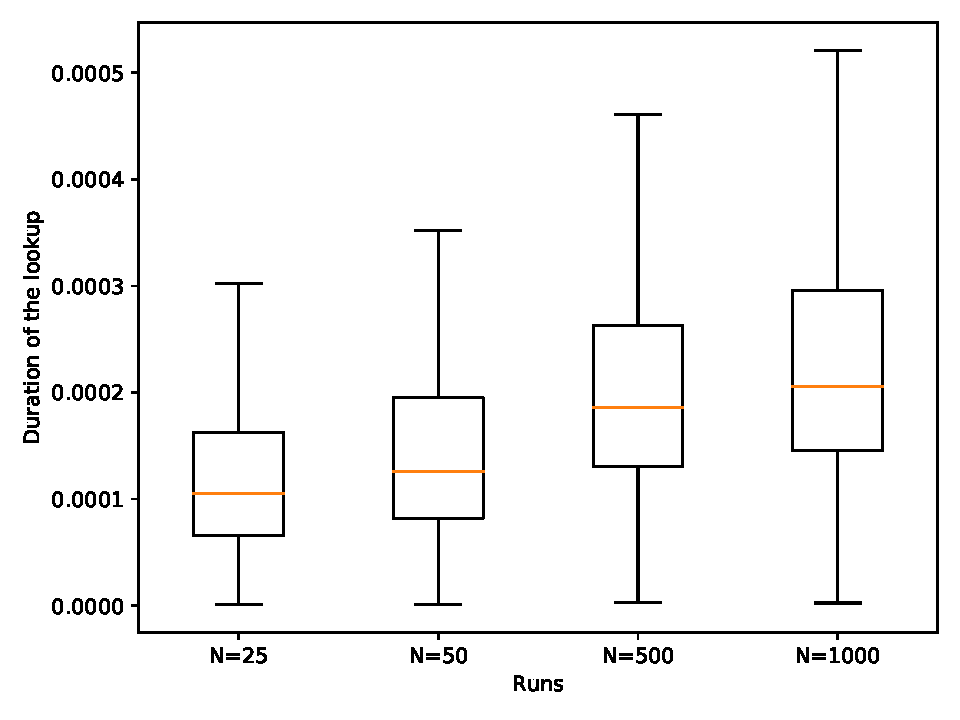
\includegraphics[width=\linewidth,clip,trim=0 0.5cm 0 0.35cm]{figures/analysis2/lookupduration_box.pdf}
		\caption{Boxplot of the lookups durations for each run}
		\label{fig:netsize0}
	\end{figure}	
	\begin{figure}[!ht]
		\centering
		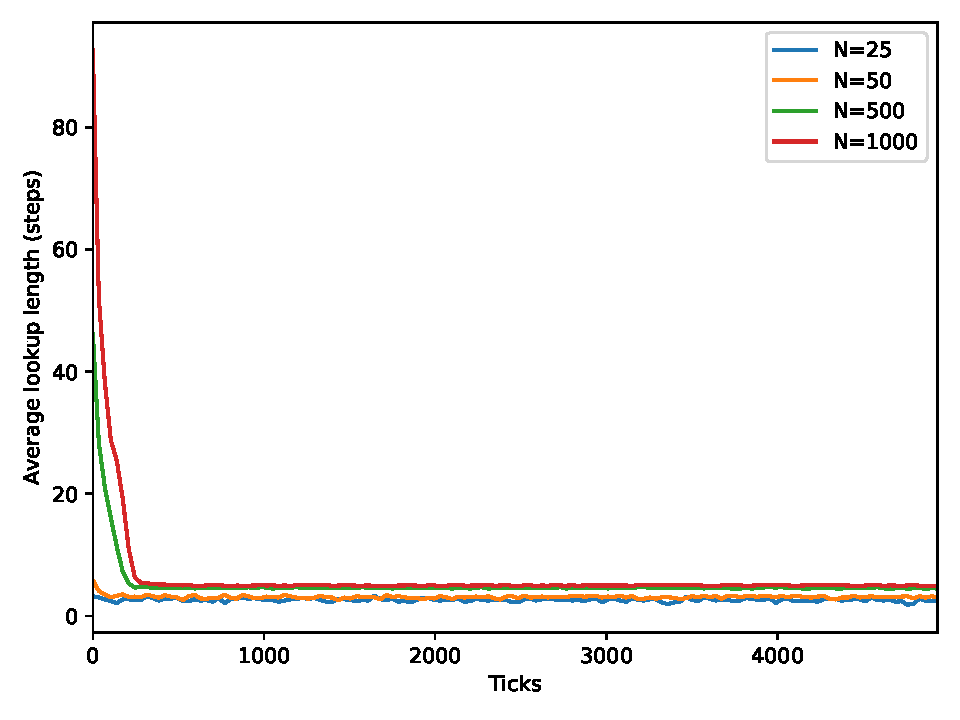
\includegraphics[width=\linewidth,clip,trim=0 0.5cm 0 0.35cm]{figures/analysis2/lookuplength_time.pdf}
		\caption{Average duration of lookups throughout each run}
		\label{fig:netsize1}
	\end{figure}
	\begin{figure}[!ht]
		\centering
		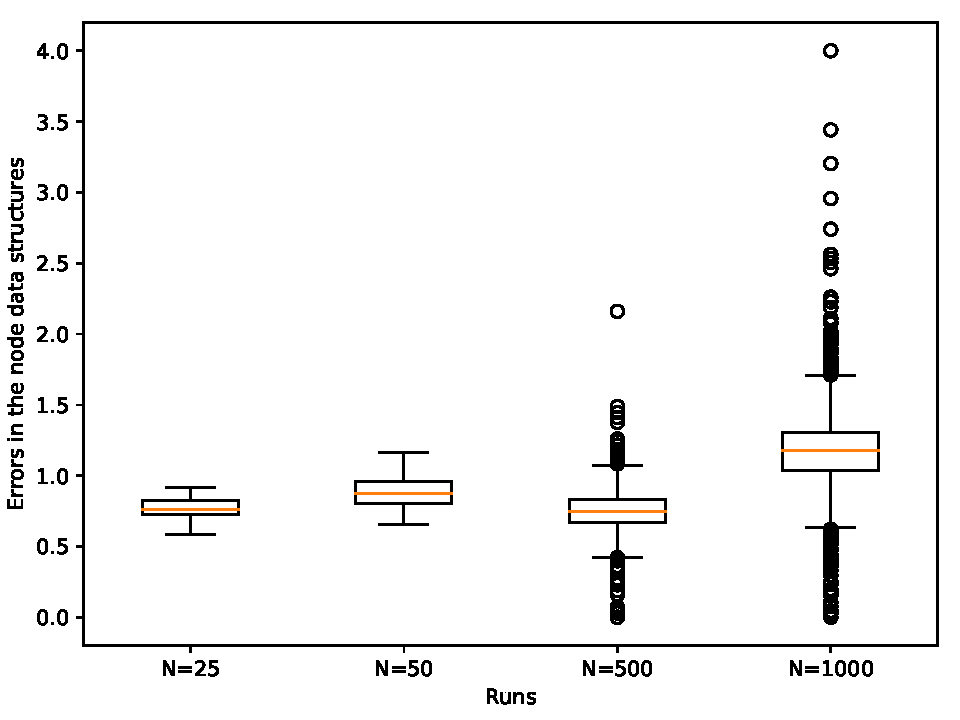
\includegraphics[width=\linewidth,clip,trim=0 0.5cm 0 0.35cm]{figures/analysis2/errors_box.pdf}
		\caption{Average number of errors in the a node data structures, i.e. caused by nodes that unsubscribed or crashed while being in the finger table and/or in the successors list of another node. Considering runs with different network sizes.}
		\label{fig:netsize2}
	\end{figure}	
		
	\begin{table}[!h]
		\caption{Variations of the default parameters for the scaling analysis runs. \texttt{R01} is omitted being the default run with no variations.}
		\label{tab:netsize_runs}
		\centering
		\begin{tabular}{lc}
			\hline
		    \multicolumn{2}{c}{\texttt{R05}}\\
			\hline
			Number of keys & 30\\
			\hline
			Hash size & 5\\
			\hline
			Initial number of nodes & 25\\
			\hline
			Successors list & 8\\
			\hline
			Join min number of nodes & 2\\
			\hline
			Leave min number of nodes & 2\\
			\hline
			Lookups per batch & 10\\
			\hline
			\hline
		    
		    \multicolumn{2}{c}{\texttt{R06}}\\
			\hline
			Number of keys & 60\\
			\hline
			Hash size & 6\\
			\hline
			Initial number of nodes & 50\\
			\hline
			Successors list & 10\\
			\hline
			Join min number of nodes & 3\\
			\hline
			Leave min number of nodes & 3\\
			\hline
			Lookups per batch & 25\\
			\hline
			\hline

			\multicolumn{2}{c}{\texttt{R07}}\\
			\hline
			Number of keys & 1000\\
			\hline
			Hash size & 10\\
			\hline
			Initial number of nodes & 500\\
			\hline
			Successors list & 15\\
			\hline
			Join min number of nodes & 5\\
			\hline
			Leave min number of nodes & 5\\
			\hline
			Lookups per batch & 250\\
			\hline
			\hline
			
			\multicolumn{2}{c}{\texttt{R01}}\\
			\hline
			\multicolumn{2}{c}{\dots}\\
			\hline
		\end{tabular}
	\end{table}		

	The plot in \Cref{fig:netsize0} shows how the duration of a lookup increases with a bigger network, however the average lookup length (\Cref{fig:netsize1}) is still very low, showing the scalability power and efficiency of the protocol.
	
	Another important observation is that the average number of errors in the node data structures is low and under control, although presenting more outliers with bigger networks, which is expected as with the corresponding larger successors lists and finger tables. This behaviour is shown in the plot in \Cref{fig:netsize2}.

	
	\subsection{Performance and quantity of keys}
	\label{subsec:keyno_analysis}
	Several runs have been executed in order to test whether the number of keys to manage influences the protocol performance (listed in \Cref{tab:keyno_runs}). The results shown in \Cref{fig:keys0,fig:keys1} shows how lookups are not impacted at all by the much greater number of keys, as the lookups duration is very similar in value and trend in all the cases, with the average number of steps corresponding almost exactly.
	\begin{table}[t]
		\caption{Variations of the default parameters for the key quantity analysis.}
		\label{tab:keyno_runs}
		\centering
		\begin{tabular}{cc}
			\hline
			\textbf{Run} & \textbf{Number of keys}\\
			\hline
			\texttt{R01} & $1000$\\
			\hline
			\texttt{R02} & $2000$\\
			\hline
			\texttt{R03} & $3000$\\
			\hline
			\texttt{R03} & $4000$\\
			\hline
		\end{tabular}
	\end{table}		

	\begin{figure}[t]
		\centering
		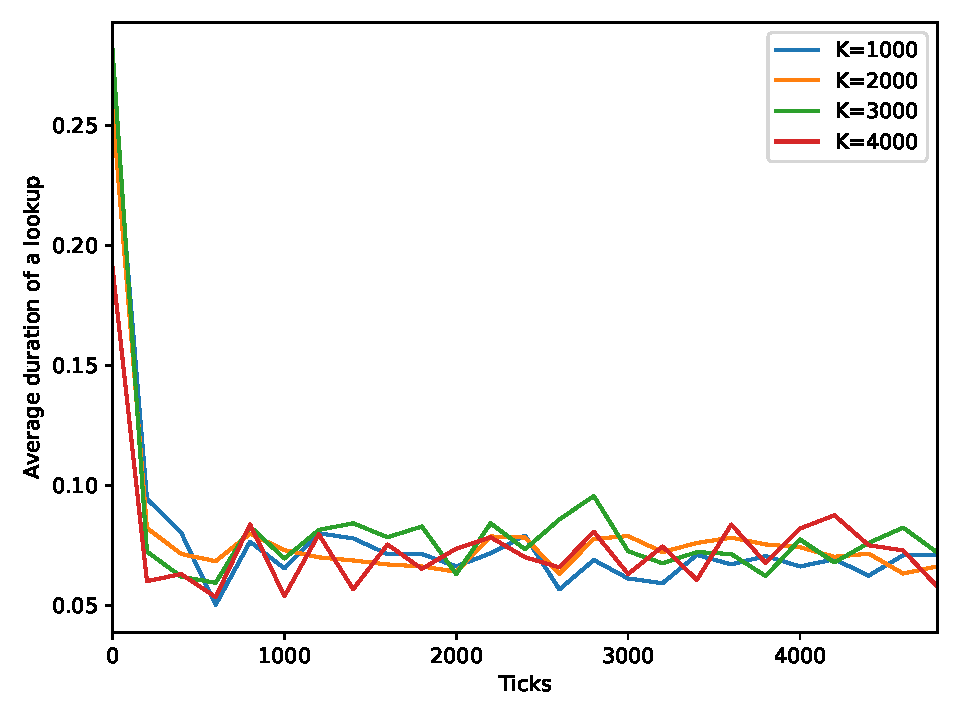
\includegraphics[width=\linewidth,clip,trim=0 0.5cm 0 0.35cm]{figures/analysis3/lookupduration_time.pdf}
		\caption{Duration of lookups throughout runs, considering different numbers of keys}
		\label{fig:keys0}
	\end{figure}
	\begin{figure}[!h]
		\centering
		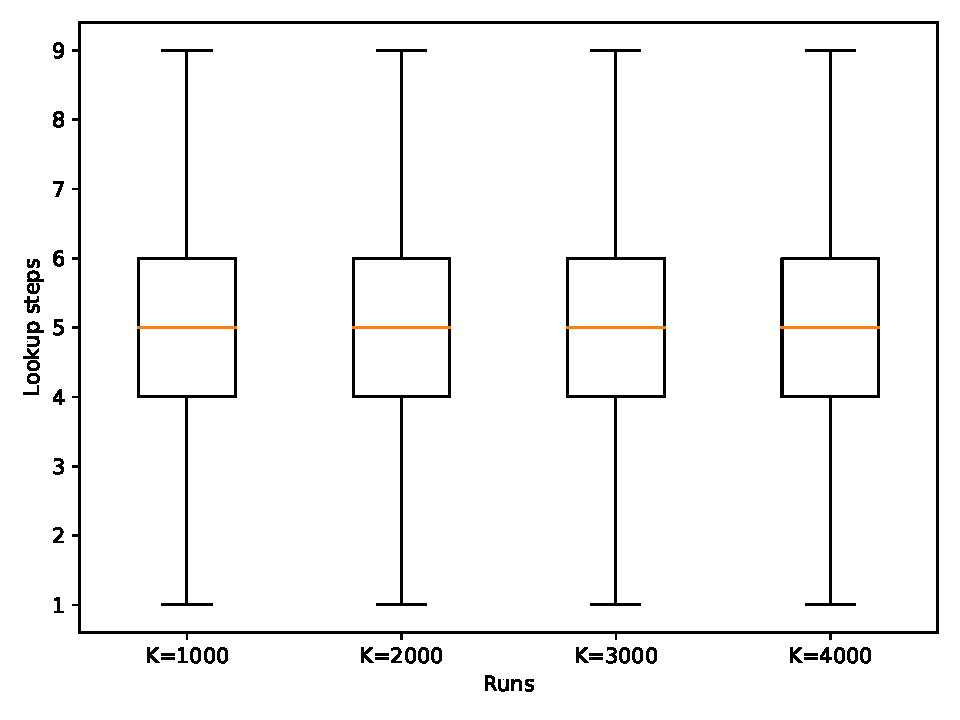
\includegraphics[width=\linewidth,clip,trim=0 0.5cm 0 0.35cm]{figures/analysis3/lookuplength_box.pdf}
		\caption{Distribution of the number of steps needed for a lookup, considering the runs with different number of keys}
		\label{fig:keys1}
	\end{figure}
	
	Another interesting analysis has been performed on the borderline case in which the lookups in the same batch requests the same exact key. Plots in \Cref{fig:keys2,fig:keys3} shows how the protocol withstands the stress of the \textit{single-key-lookup}~(\textit{skl}) both for what concerns the number of steps and the lookup duration, the latter presenting some spikes probably due to some node crashing with a yet not distributed information needed for some lookup.\\

	\begin{figure}[ht]
		\centering
		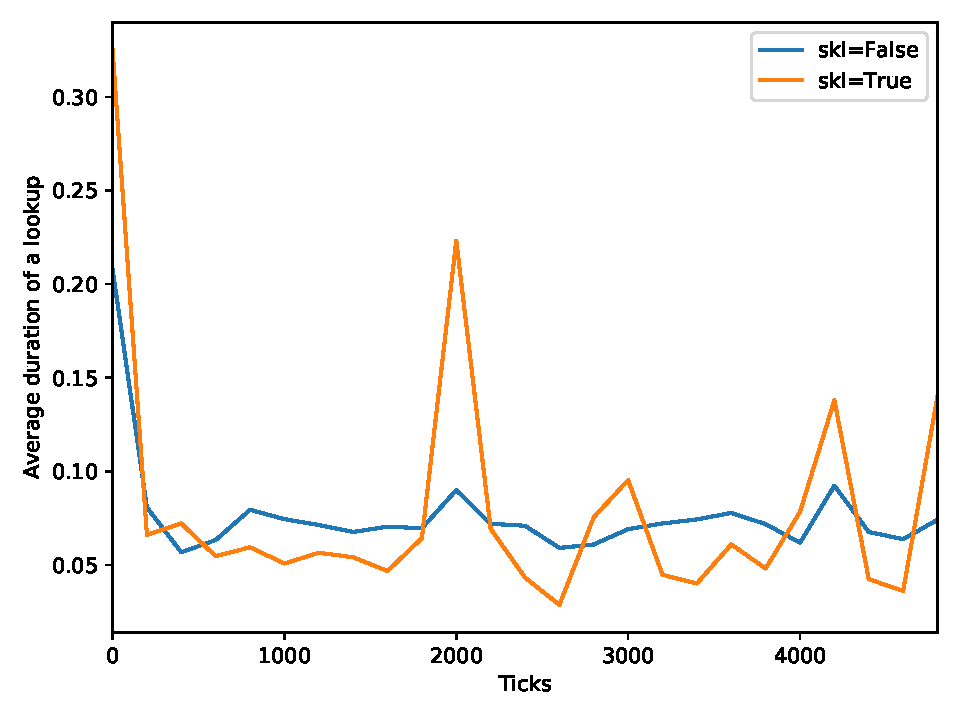
\includegraphics[width=\linewidth,clip,trim=0 0.5cm 0 0.35cm]{figures/analysis3/skl_lookupduration_time.pdf}
		\caption{Duration of lookups throughout runs, considering the single-lookup case (skl=True)}
		\label{fig:keys2}
	\end{figure}
	\begin{figure}[ht]
		\centering
		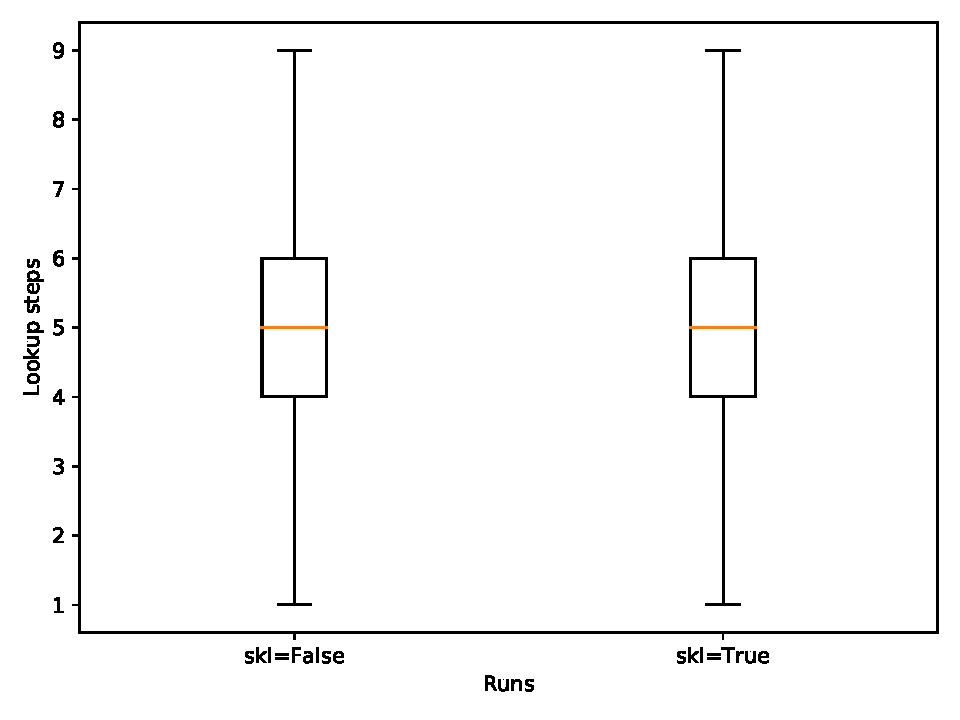
\includegraphics[width=\linewidth,clip,trim=0 0.5cm 0 0.35cm]{figures/analysis3/skl_lookuplength_box.pdf}
		\caption{Distribution of the number of steps needed for a lookup, considering the single-lookup case run (skl=True)}
		\label{fig:keys3}
	\end{figure}
	
	Finally, it's important to check how the average quantity of keys managed by a node changes with different network sizes. \Cref{fig:keys4} shows how this value is distributed for the runs in \Cref{tab:netsize_runs}: considering that the total number of keys is balances wrt the number of nodes of the configuration, the expectation is to have similar distributions, which is actually observed in the plot. 
	\begin{figure}[!t]
		\centering
		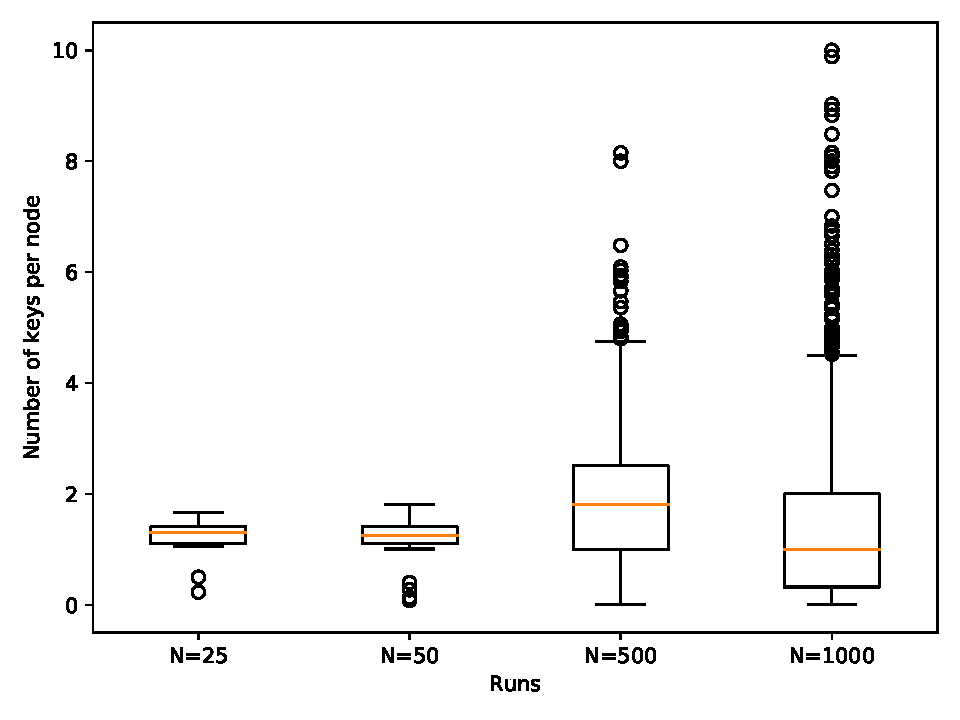
\includegraphics[width=\linewidth,clip,trim=0 0.5cm 0 0.35cm]{figures/analysis3/keyspernode.pdf}
		\caption{Number of keys managed by a node with different network sizes.}
		\label{fig:keys4}
	\end{figure}	

	\subsection{Plotting script usage}
		The plots for the performed analyses has been generated with the \texttt{chord\_analyzer.py} script, which was implemented for this purpose. The arguments usage is explained in \Cref{tab:script}.
		\begin{table}[!h]
			\centering
			\begin{tabular}{cl}
				\hline
				\textbf{Arg} & \textbf{Usage}\\
				\hline
				1 & Base folder where the Repast logging files are located\\
				\hline
				2 & Requests for the scripts, comma separated. \textit{loadnodes} and \textit{loadlookups} respectively loads the Lookup and Node datasets. \textit{all} generates all the implemented plots possible with the loaded datasets, which can also be selectively chosen with the corresponding names ("lookupduration\_time", lookupduration\_box", errors\_time", errors\_box", timeouts\_time", timeouts\_box", nodescontacted\_time", nodescontacted\_box", lookuplength\_time", lookuplength\_box", keyspernode", "nodesup\_time", failedlookups")\\
				\hline
				3 & Log files index (XX) to load, comma separated. Expecting Lookup\_XX and Node\_XX file as data sinks names\\
				\hline
				4 & \\
				\hline
				5 & \\
				\hline
				6 & \\
				\hline
			\end{tabular}
		\end{table}

	\clearpage
	\printbibliography
\end{document}











































